% Template for Elsevier CRC journal article
% version 1.2 dated 09 May 2011
%------------------------------------------

%% The '3p' and 'times' class options of elsarticle are used for Elsevier CRC
%% The 'procedia' option causes ecrc to approximate to the Word template
\documentclass[5p,times,procedia]{elsarticle}
\flushbottom



%% The `ecrc' package must be called to make the CRC functionality available
\usepackage{ecrc}
\usepackage{amsmath}

% JO bibliography:
%\usepackage[sorting=none]{biblatex} %biblatex -nope!
%\addbibresource{Bibliography.bib}   %biblatex -nope!
%\usepackage{natbib}                 %natbib.  -nope!
%\bibliographystyle{unsrtnat}        %unsrtnat -nope!

% Jo color definition:
\usepackage{xcolor}
\definecolor{notecolor}{rgb}{0.16, 0.67, 0.53}

% JO note environment:
\newenvironment{note}{%
	\noindent
    \color{notecolor}%
}{%
    \par\medskip%
}


\usepackage{siunitx} %SI-units
\usepackage{eurosym} %euro symbol
%\usepackage{hyperref}



%% set the volume if you know. Otherwise `00'
\volume{00}

%% set the starting page if not 1
\firstpage{1}

%% Give the name of the journal
\journalname{Procedia CIRP}

%% Give the author list to appear in the running head
%% Example \runauth{C.V. Radhakrishnan et al.}
\runauth{J. Kimmle et al.}

%% The choice of journal logo is determined by the \jid and \jnltitlelogo commands.
%% A user-supplied logo with the name <\jid>logo.pdf will be inserted if present.
%% e.g. if \jid{yspmi} the system will look for a file yspmilogo.pdf
%% Otherwise the content of \jnltitlelogo will be set between horizontal lines as a default logo

%% Give the abbreviation of the Journal.
\jid{trpro}

%% Give a short journal name for the dummy logo (if needed)
%\jnltitlelogo{Transportation Research}

%% Hereafter the template follows `elsarticle'.
%% For more details see the existing template files elsarticle-template-harv.tex and elsarticle-template-num.tex.

%% Elsevier CRC generally uses a numbered reference style
%% For this, the conventions of elsarticle-template-num.tex should be followed (included below)
%% If using BibTeX, use the style file elsarticle-num.bst

%% End of ecrc-specific commands
%%%%%%%%%%%%%%%%%%%%%%%%%%%%%%%%%%%%%%%%%%%%%%%%%%%%%%%%%%%%%%%%%%%%%%%%%%

%% The amssymb package provides various useful mathematical symbols
\usepackage{amssymb}


% if you have landscape tables
\usepackage[figuresright]{rotating}
%\usepackage{harvard}
% put your own definitions here:x
%   \newcommand{\cZ}{\cal{Z}}
%   \newtheorem{def}{Definition}[section]
%   ...

% add words to TeX's hyphenation exception list
%\hyphenation{author another created financial paper re-commend-ed Post-Script}

% declarations for front matter

\usepackage[bookmarks=false]{hyperref}
    \hypersetup{colorlinks,
      linkcolor=blue,
      citecolor=blue,
      urlcolor=blue}


\begin{document}
\begin{frontmatter}



%% Title, authors and addresses

%% use the tnoteref command within \title for footnotes;
%% use the tnotetext command for the associated footnote;
%% use the fnref command within \author or \address for footnotes;
%% use the fntext command for the associated footnote;
%% use the corref command within \author for corresponding author footnotes;
%% use the cortext command for the associated footnote;
%% use the ead command for the email address,
%% and the form \ead[url] for the home page:
%%
%% \title{Title\tnoteref{label1}}
%% \tnotetext[label1]{}
%% \author{Name\corref{cor1}\fnref{label2}}
%% \ead{email address}
%% \ead[url]{home page}
%% \fntext[label2]{}
%% \cortext[cor1]{}
%% \address{Address\fnref{label3}}
%% \fntext[label3]{}

\dochead{57th CIRP Conference on Manufacturing Systems 2024 (CMS 2024)}

\title{Digital twin based online material defect detection for CNC-milled workpieces}

%% use optional labels to link authors explicitly to addresses:
%% \author[label1,label2]{<author name>}
%% \address[label1]{<address>}
%% \address[label2]{<address>}



\author[a,b]{Johannes Kimmle} 
\author[a,c]{Dominik Lucke\corref{cor1}}%$\ast$}} %{cor1}
\author[b]{Konrad von Leipzig}
%\ead{author@institute.xxx}

\address[a]{ESB Business School, Reutlingen University, Alteburgstra\ss e 150, 72762 Reutlingen, Germany}
\address[b]{Department of Industrial Engineering, Stellenbosch University, Joubert Street, Stellenbosch, 7600, South Africa}
\address[c]{Fraunhofer Institute for Manufacturing Engineering and Automation IPA, Nobelstra\ss e 12, 70569 Stuttgart, Germany}

\aucores{* Corresponding author. Tel.: +49-7121-271-5005; fax: +49-7121-271-90-5005; E-mail address: dominik.lucke@reutlingen-university.de}

\begin{abstract}
Reliable lot-size-one compatible online quality monitoring for CNC machined parts remains elusive.
To address this challenge, our approach aims to bridge the current gap in research by developing a cost-effective and reference-independent monitoring concept for material defect detection in CNC-machined parts. This paper presents a novel digital twin-based method, utilising machining vibrations and a g-code-based encoding of the cutting process. The objective is to detect material defects, such as blowholes, without the need for individual workpiece references. The proposed method aims to reduce barriers to entry, minimise waste, and enhance machine productivity by enabling automated early online quality control. To develop and validate the model, we generate a new dataset combining machining vibration with technological context data such as chip-shape. We demonstrate the feasibility and potential of the approach in a job shop setting on a 3-axis CNC mill.
\end{abstract}

\begin{keyword}
 Online process monitoring \sep Material defect detection \sep Digital Twin

%old: Monitoring \sep Machining \sep Material defects \sep Vibrations \sep Lot size one

%% keywords here, in the form: keyword \sep keyword

%% PACS codes here, in the form: \PACS code \sep code

%% MSC codes here, in the form: \MSC code \sep code
%% or \MSC[2008] code \sep code (2000 is the default)

\end{keyword}
\cortext[cor1]{Corresponding author. Tel.: +49-7121-271-5005; fax: +49-7121-271-90-5005; E-mail address: dominik.lucke@reutlingen-university.de}

\end{frontmatter}


%=====================================================================
%=====================================================================
\section{Introduction}\label{Sec_Introduction}


The manufacturing industry is undergoing a paradigm shift, transitioning from a focus on responsiveness to a market-of-one, deemed Mass Individualisation\cite{Lu.Xu.ea2020} or Mass Personalisation \cite{Qin.Lu2021}. This entails the production of custom-made products while maintaining the low unit costs traditionally associated with mass production.
In response, there has been a global push towards smart manufacturing characterized by autonomous operations enabled by advanced sensing, data processing, and decision-making technologies. \cite{Gu.Koren2022, Lu.Morris.ea2016}

Within this context, reducing lot sizes in job-shop settings becomes imperative,



\begin{note}
... weg damit...\\
Within this context, reducing lot sizes in job-shop settings becomes imperative, and additive manufacturing (AM), particularly 3D printing, emerges as a promising solution due to its autonomy and versatility.
However, despite its advantages, AM still falls short compared to traditional techniques like CNC milling in aspects such as dimensional accuracy, mechanical properties, material variety, and surface quality \cite{Chen.Lin2017, Schmidt2016}.
CNC milling, therefore, remains pivotal, presenting not only significant potential but also high necessity for optimisation due to its complex nature of underlying processes that result in lower process resilience and robustness compared to AM.
\end{note}


%\vspace*{8pt}
\vspace*{-\baselineskip}
\begin{nomenclature}
\begin{deflist}[AAA]%number of letters
\defitem{CNC}\defterm{Computerised Numerical Controled (machine tool)}
\defitem{AM}\defterm{Additive Manufacturing}
\defitem{ML}\defterm{Machine Learning}
\end{deflist}
\end{nomenclature}%\vskip24pt


A monitoring system that utilises deep process context (e.g. technological, geometric, or material property data) to generate reference agnostic - lot size one capable - process status insights, would ready CNC mills for the Mass Personalisation paradigm shift.

Such a workpiece-centred monitoring system, which detects material defects or operator errors (e.g. wrong material, or part clamping errors) during normal machining, can increase process efficiency \& reliability, reduce waste, and enable higher product quality.  

To achieve economic efficiency and general market accessibility, this lot-size-one capable system must be easy to integrate, machine-agnostic, and relatively low-cost.


 
%=====================================================================
\section{Related work}\label{Sec_RelatedWork}


%Machine tool and machine tool control munafacturers integrate all kind of monitoring capabilities in their products. Modern CNC mills are usually factory-fitted with spindle and axis drive energy meters where spindle tourque and axis resistance can be estimated from.

%Most of these focus on tool wear, surface finish optimisation, or machine maintenance. 
%Holistic process specific monitoring especially of the workpiece is rarely employed on today's shop floors or in current research.\\

%Almost exclusively CNC monitoring is focused on tool condition monitoring (especially tool wear and breakage), surface finish quality (including chatter), and machine health monitoring (within the scope of predictive maintenance) .
Predominantly, CNC monitoring is focused on tool condition monitoring, particularly detecting tool wear and breakage, ensuring surface finish quality, including mitigating chatter, and monitoring machine health for predictive maintenance purposes \cite[p.2727]{Kuntoglu.Salur.ea2021}.
The following sensors are in use for CNC monitoring and are rated by investment cost and information value (see: Table \ref{Tab_Sensors}).
\vspace*{-.5\baselineskip}


\begin{table}[h]
\footnotesize
\caption{Sensors according to signals and properties \cite[according to][p.2725]{Kuntoglu.Salur.ea2021}}
\label{Tab_Sensors}

\begin{tabular*}{\hsize}{@{\extracolsep{\fill}}lll@{}}
\toprule
Sensor & Level of investment cost & Extent of signal accuracy\\ && and information value\\
\colrule
Dynamometer    & $\bullet$\hspace{.5mm}$\bullet$\hspace{.5mm}$\bullet$\hspace{.5mm}$\bullet$\hspace{.5mm}$\bullet$\hspace{.5mm}   & $\bullet$\hspace{.5mm}$\bullet$\hspace{.5mm}$\bullet$\hspace{.5mm}$\bullet$\hspace{.5mm}$\bullet$\hspace{.5mm}\\
Accelerometer  &   $\bullet$\hspace{.5mm}$\bullet$\hspace{.5mm}$\bullet$\hspace{.5mm}$\bullet$\hspace{.5mm}   &  $\bullet$\hspace{.5mm}$\bullet$\hspace{.5mm}$\bullet$\hspace{.5mm}\\
AE             & $\bullet$\hspace{.5mm}$\bullet$\hspace{.5mm}$\bullet$\hspace{.5mm}$\bullet$\hspace{.5mm}     & $\bullet$\hspace{.5mm}$\bullet$\hspace{.5mm}$\bullet$\hspace{.5mm} \\
Current/power  & $\bullet$\hspace{.5mm}      & $\bullet$\hspace{.5mm}  \\
Temperature    & $\bullet$\hspace{.5mm}$\bullet$\hspace{.5mm}$\bullet$\hspace{.5mm}      & $\bullet$\hspace{.5mm}$\bullet$\hspace{.5mm}  \\
Sound          & $\bullet$\hspace{.5mm}      & $\bullet$\hspace{.5mm}  \\
\botrule 
\end{tabular*}
\end{table}

\vspace*{-.5\baselineskip}
Dynamometers commonly utilise all six spatial axes (three translatory and three rotatory) to capture force profiles at high sampling rates, with higher rates correlating with increased cost.
Vibrations measured by accelerometers refer to the oscillatory motion of an object or system around an equilibrium position ($f_{acc}$ $\lesssim$ 10 kHz).
AE refers specifically to the release of stress waves or energy due to internal changes or deformation within a material. AE is difficult to measure in lower frequencies; usual frequencies band is: 20 kHz $\lesssim$ $f_{AE}$ $\lesssim$ 500 kHz. \cite{Jozwik.Mika2015, Sun.Hu.ea2020}

Current/power is measured from the drive unit of the spindle (and translates ruffly into spindle tourque) and is therefore extremely cost effective.
Temperature, mostly measured via thermal imaging cameras, lack high sample rates (due to low frame rates), and suffer from delays and perspective obstacles. 



\subsection{Similar monitoring solutions}
\vspace*{-\baselineskip}


\href{https://www.matta.ai/greymatta}{Matta's Grey-1 model} as shown in their paper \cite{Brion.Pattinson2022} demonstrates AM process monitoring on fused layer deposit 3D printers, based on an automated deep process understanding. 
They trained a multi head transformer model on labeled images; labels such as: extrusion speed, layer thickness and hotend temperature. They are able to detect extrusions errors (which translate into material defects), or adjust printing parameters fully autonomously for unseen material. \cite{Brion.Pattinson2022}


\cite{Pfirrmann.Baumann.ea2021} investigates the cutting forces measured by a (6-axis) dynamometer in the micromanufacturing of Ti6246 alloy by comparing them with theoretically calculated forces, to detect material defects such as blowholes.
This approach is in theory lot size one capable because the force measurement is not compared to a previsouly manufacured 1:1 reference, but rather is based on experimental measurements and a geometric physics-based process simulation. 
It is concluded that the accuracy of the calculated force and the insufficient change in amplitude between normal and defect machining are too low to achieve automated detection. \cite[p.169]{Pfirrmann.Baumann.ea2021} 

While dynamometer force measurements offer the highest signal accuracy and information value due to their direct measurement method and process proximity \cite[]{Korkmaz.Yasar.ea2020}, they are expensive (\euro $10^4$ magnitude), difficult to set up, and usually not feasible for production environments (compare Table \ref{Tab_Sensors}).

Qass's Optimizer 4D, an off-the-shelf AE-based general-purpose inspection system, addresses the problems of dynamometers described above, at the cost of reduced signal accuracy. The system is still expensive, but it comes with out-of-the-box spectral pattern recognition, which enables reference-dependent material defect detection, thus is not lot size one capable. \cite[p.5]{Szulewski.Sniegulska-Gradzka2017}

\vspace*{.5\baselineskip}
\noindent The current research gap in this field is concluded as follows: \label{gap}
\vspace*{-\baselineskip}
\begin{itemize}
	\item Research in online CNC workpiece quality monitoring remains relatively underexplored.
	\item Material defect detection represents a particular under-researched subfield.
	\item Only one single paper has been identified thus far that addresses reference-independent defect monitoring within this domain. % (and did not suceed, see \cite[p.5]{Szulewski.Sniegulska-Gradzka2017}).
\end{itemize}










%=====================================================================
\section{Aproach}\label{Sec_Aproach}

Digital twins provide a solution to fullfill the requirements listed at the end of section \ref{Sec_Introduction} in the scope of the research gap concluded in section \ref{Sec_RelatedWork}, by enabling the combination of cost-effective retro-fit sensors that don't disturb machining and an encoding of the cutting process serving as contextual refference, to enable effective lot-size one monitoring.

\begin{note}
alternativ...

	Digital twins offer a solution to meet the requirements outlined at the end of Section \ref{Sec_Introduction} and address the research gap identified in Section \ref{Sec_RelatedWork}. This is achieved by integrating affordable retrofit sensors that do not interfere with machining and encoding the cutting process for contextual reference, enabling efficient monitoring tailored to individual production runs.
\end{note}

\subsection{Physical quanitity to monitor}
\vspace*{-\baselineskip}
Vibrations measured via accelerometers or Acoustic Emission (AE) sensors form a great compromise between ease of installation \& cost, and signal accuracy \& information value. While Dynamometers entail greater information value, their high cost and poor mountability don't make them viable for general monitoring. Other options such as "current/power" "temperature" or "sound" hold lower information value and are therefore not considered.

The easily and cheaply achievable high sampling rates of vibration measuremnts are an enormous advantage when zooming in in the timedomain and analysing each cutting event (cutting edge engagement). As the paper \cite{Pfirrmann.Baumann.ea2021} shows that especially smaller/micro material defects affect machining forces for just a few edge engagements, lasting in total a few microseconds.

\subsection{Machining-context features}
\vspace*{-\baselineskip}

Key aspect of our aproach is to substitute a 1:1 reference of the same part manufactured prior, by general machining and cutting conditions and circumstances for each point in time in the manufacturing process, we call this data: context.
To design our context features, we came up with 3 questions.

\vspace*{-.5\baselineskip}
\begin{enumerate}
	\item \textit{What factors influence the cutting process?}
	\vspace*{-\baselineskip}
	\begin{itemize}
		\item workpiece -geometry, -clamping, -material characterstics (e.g. e-module)
		\item tool -type (shape), -coating (surface), -cutting fluid
		\item machine -kinemantics, -stiffness, -sub componenent noise
		\item cutting process on chip level (e.g. rake angle)
		\item generall milling process (e.g. cutting speed: $v_c$)
		\item others: temperature, chip extraction, direction, etc.
	\end{itemize}	
	\vspace*{-\baselineskip}
	The above factors affect the cutting process, some directly by influencing the load on the material being removed, ultimately resulting in a change in the virbation pattern. Others affect the process indirectly through resonance, e.g. slender workpiece geometries are excited at their natural frequency.
	
	\vspace*{.5\baselineskip}
	\item \textit{How can the process be described as universally as possible by these factors?}\\
	Some factors can't be generalised, or are not feasable to do so. Those factors stay as static features that need specific learning later.
	Incomprhesible features e.g. "specific machine" can't be generalised because of their complex nature, therefore each machine needs custom learning.
	Other features are not feasable to generalize because they would make the medel too complex: e.g. material characterisitcs can be explained by more general features such as hardness, tensile strength, etc. Due to the high number of material features, we decided to custom train each material.
	We have identified the following static features on which later learning is based:
	material, machine, clamping/fixture, tool type, and cutting fluid.
	
	Factors that are generalisable - where comprehensible and detachable features with general predication can be derived from - are prefered and form the backbone of deep process insights. E.g. cutting speed $v_c$, is machine, material and tool independent while having substential influence on the cutting process, ultimatly influencing sensor signal patterns.
	
	Factors that require specifc sensors in order to be captured, such as temperature, are excluded from the model to keep complexity manageable.
	
	\vspace*{.5\baselineskip}
	\item\label{Q3} \textit{How can these factors be modelled as mathematically independent (uncoupled, lower-dimensional) coefficients?}\\
	To achieve high quality training data interdependence or correlation among features is to be avoided.
	Most classical technological paramters are interdependent: e.g. infeed $a_p [mm]$ is dependent on tool diamter $d [mm]$, that means by changing the tool to a bigger diameter, the ratio from $a_p$ and $d$ changes. To fix this $a_p$ needs dimensional reduction: from $a_p [mm]$ to $a_p / d [\%]$ removing the interdependence of $d$. Feed rate $f$ is dependent on cutting speed $v_c$ and tool diameter $d$. Uncoupled $f$ translates into feed rate per tooth $f_z$.
	
	We found the following independent coeffiecients:
	tool diameter $d$, cutting speed $v_c$, infeed percent $a_{p\%}$, cutting depth $a_e$, tool edge number $z$, direction, milling mode (climb or up-cut), spindle speed $n$
		
	Additional features are modelled to better describe the cutting context such as: contact arc (angle of attack where tool is in contact with workpiece), arc direction (direction vector of contact arc), chip volume, cutting frequency, 
	
	Not all the considered factors can be fully modelled, so there is always some loss of information.
	Whether the remaining information is sufficient to model the cutting context is analysed in our proof-of-concept implementation.
\end{enumerate}

The final context features are a mix of static features concluded in question 2 (e.g. material), independent coefficients (e.g. feed rate per tooth), as well as additionally modeled features (e.g. contact arc) from question 3.





\subsection{Concept architecture}\label{Sec_ConceptArchitecture}
\vspace*{-\baselineskip}
The general aproach to the lot size one capable material defect monitoring integrates dirctly into common pre-existent production interfaces to enable easy machine agnostic retrofitting. The full concept architecure is shown in Fig. \ref{Fig_ConceptDiagram}.
The diagram centers around the "CNC Mill" including its "CNC Controler" in the bottom center. The process steps highlighted in bright green colour represent the standard information flow on the shop floor for CNC machines - no monitoring -just the pre-existent "Conventional Shop Procedure".
The monitoring system integrates right on top of this procedure which can be subdiveded into four "Monitoring Procedures" (grey boxes): "Signal Acquisition \& Preperation", "Context Acquisition \& Generation", "Signal Context Overlay", and "Contextualised Classification".

Inside those procedure boxes (bright green and grey) are dark blue coloured "Process Steps", specific functions that process information. Information flows in and out of these dark blue "Process Steps", this flow and exchange of information is visualised with arrows and rounded boxes in turquoise colour, we called them "Exchanged Inforamtion".
See the diagram for details.

To detect defects while machining, the architecture is designed to be real-time capable. The "Conventional Shop Proecdure" - except milling itself - and "Context Acquisition \& Generation" procedures are deterministic and therefore can be calculated beforehand, all other procedures must be real time capable, including "Signal Acquisition", "Signal-Context Overlay" and the "Contextualised Classification".

\begin{figure*}[t]
    \centering
    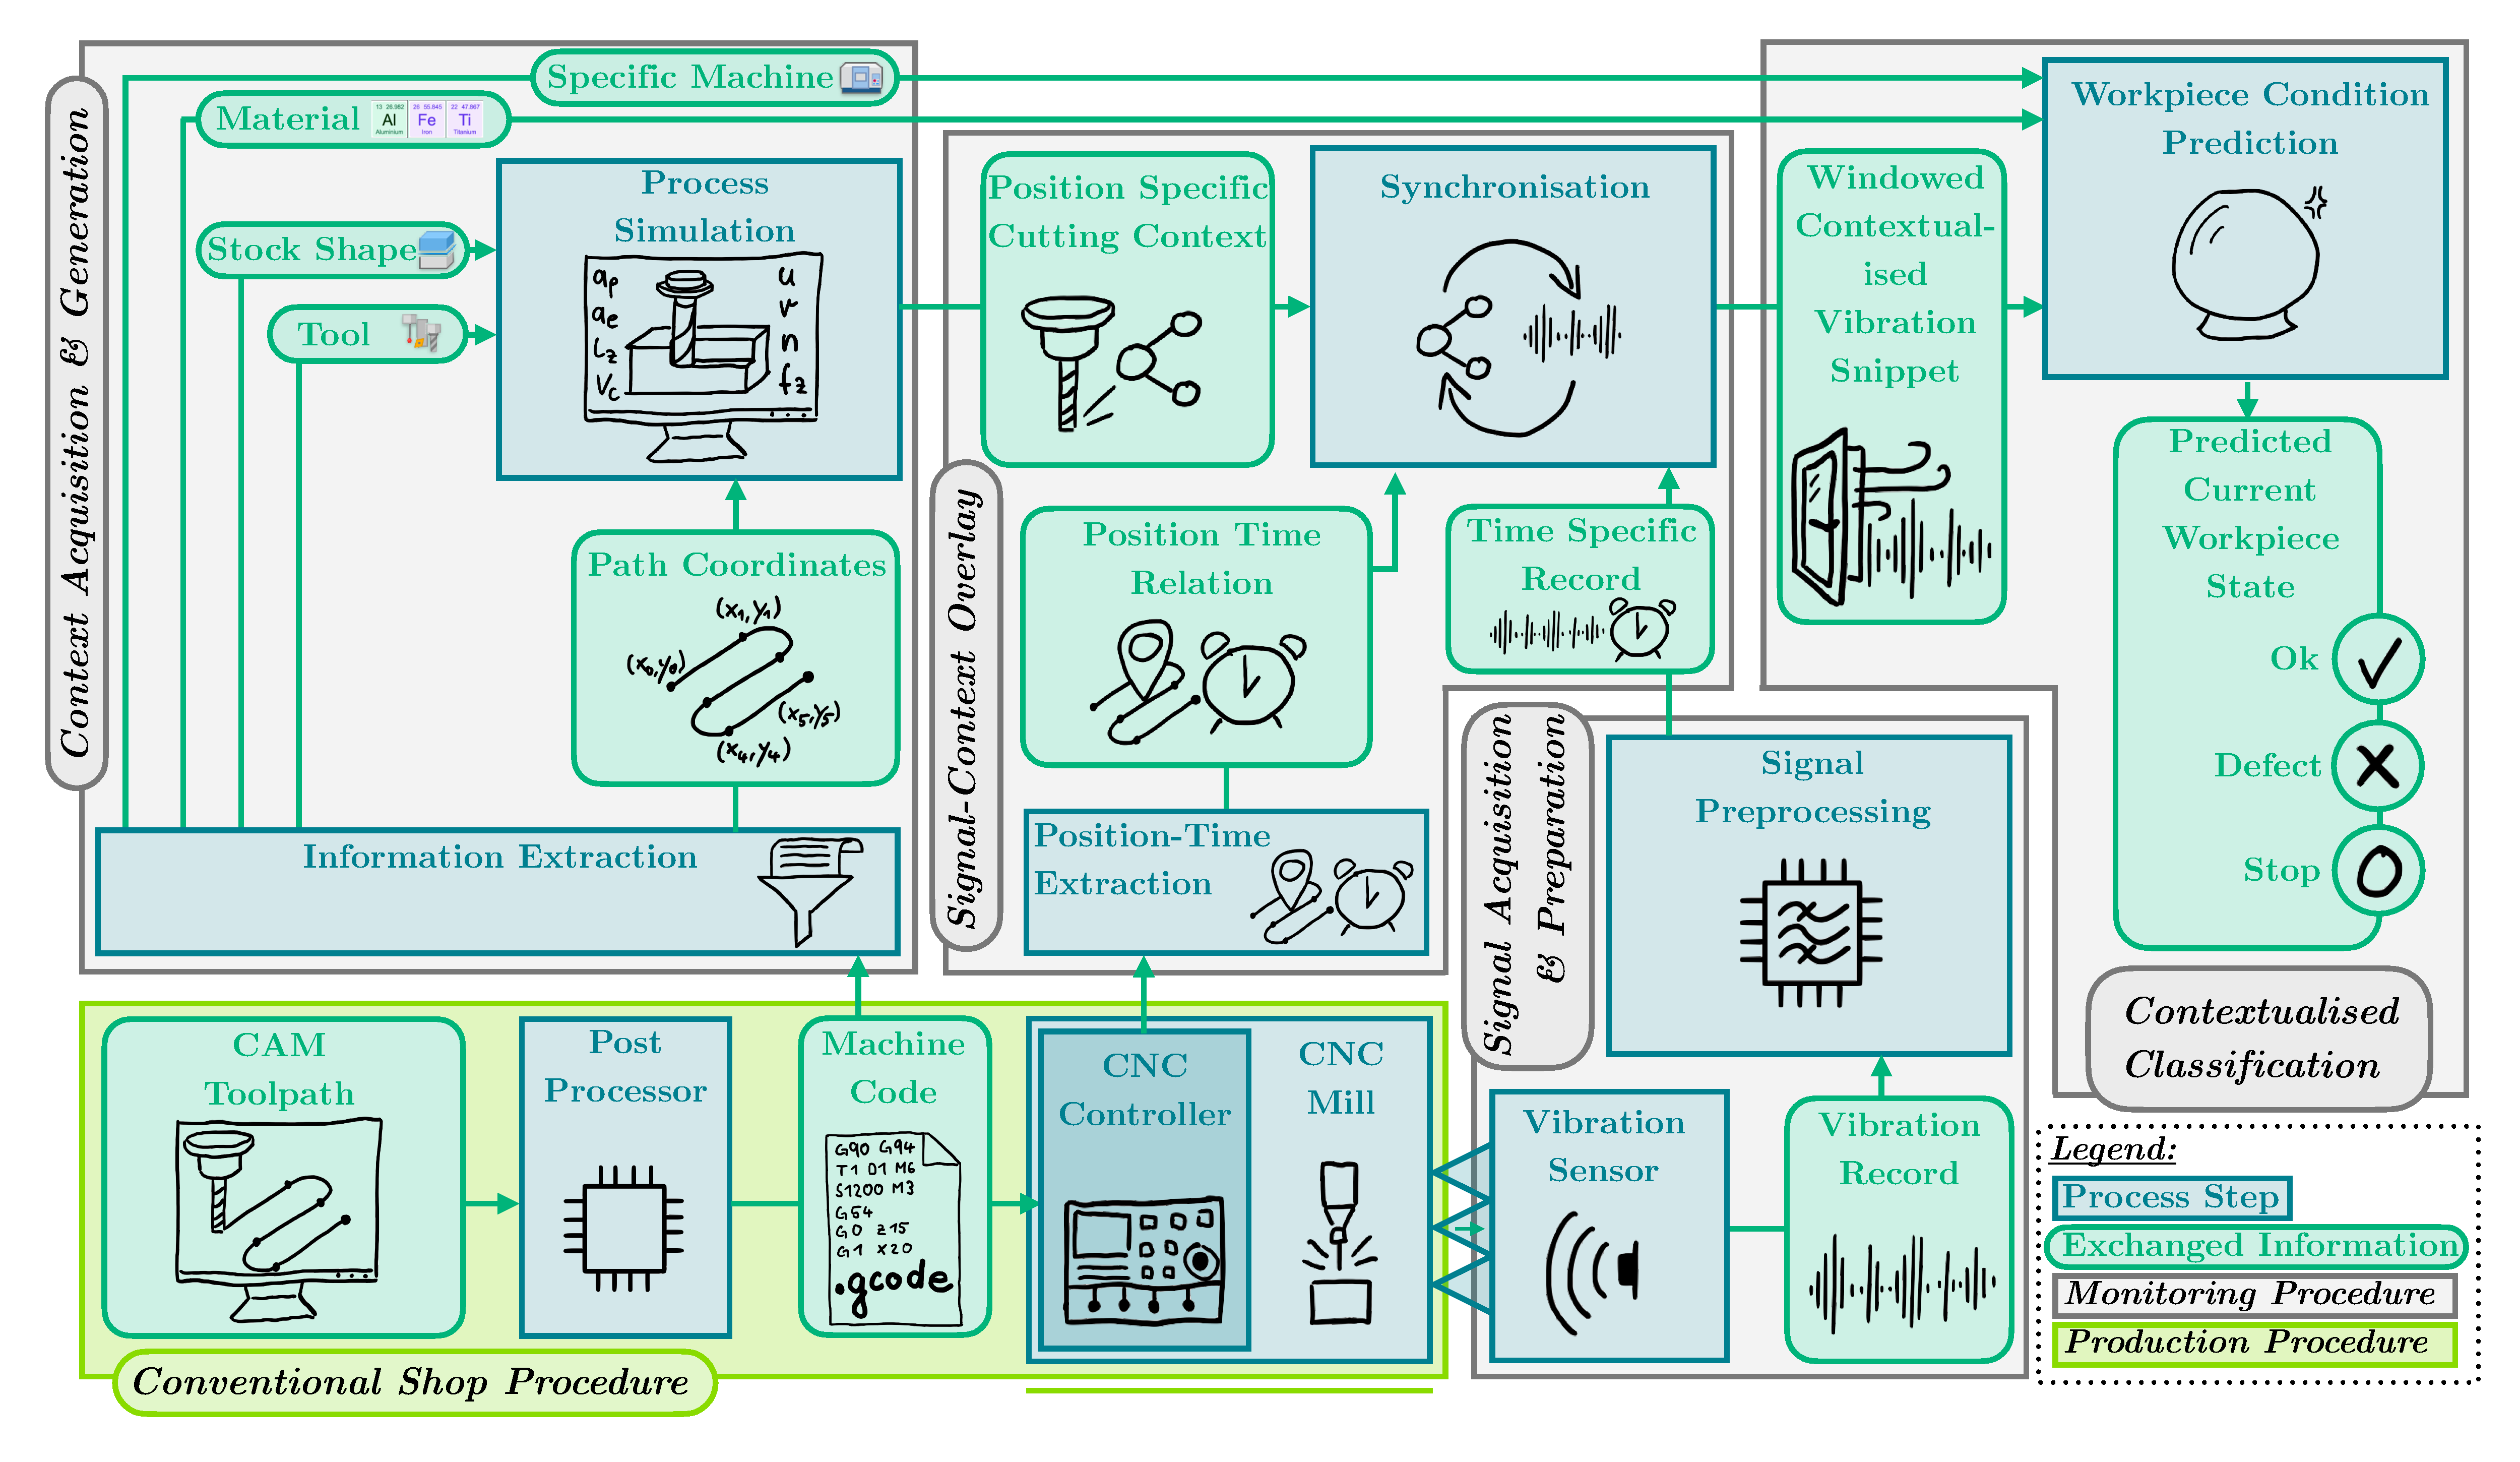
\includegraphics[width=0.99\linewidth]{ConceptDiagram.pdf}
    \caption{High-Level Concept}
    \label{Fig_ConceptDiagram}
\end{figure*}
 


\subsection{ML architecture ???}
\vspace*{-\baselineskip}
\begin{note}
	- diagram mit high level ML (konzeptionell) -eher nett!\\
	- realtime capability /\\
	- model diagram: con2D to MLP
	- seperate training (1. abstraction, 2. classifacation
\end{note}


As explained in section \ref{Sec_ConceptArchitecture}, "Contextual Classification" must be real-time capable. As part of that procedure the ML architecture is chosen accordingly. This means that in production the trained model is fed constantly with a fixed length of overlapping short vibration snippets ($\sim0.5 s$ duration) and according context data specific to each vibration snippet. 

As shown in Fig. \ref{Fig_MLArcicture} 



%=====================================================================
\section{Implementation}
\subsection{Proof of concept}
\vspace*{-\baselineskip}
\begin{note}
from full design concept to simplified proof of concept.
DoE,  

welche context feature können heraus vereinfacht werden? - Maschinentyp=1, Werkstoff=1 ...
\end{note}


To validate the concept (from Chap. \ref{Sec_ConceptArchitecture}) a simplified version is implemented as prototype to answer if reference independent defect detection based on context data is possible and if so to which extent.

Contextual features essential for the production concept, yet easily abstracted, are omitted to prioritise features with influence-characteristics that are challenging to assess beforehand. For example, if reliable defect classification works on one type of machine, it is probable to perform similarly on another machine when trained on data specific to said machine.
Given the rationale of the example above, features such as 'machine-type' and 'material' are excluded from the prototype's contextual data.
The feature 'stock shape' is believed to influence Eigen-frequencies, particularly on slender parts. To ensure explicit testability, only non-slender geometries are retained, leading to the rationalisation of the 'stock shape' feature.
An example of a feature deemed relevant for the prototype, owing to the difficulty of generalizing it beforehand, is the 'contact-arc'.


DoE, static


\#Setup???

To prevent data imbalance, ensure broad coverage of context parameter values \& combinations, and achieve a clean, reproducible dataset, a Design of Experiment (DoE) approach is employed. This involves creating a static dataset by defining the span of parameter values and their combinations as sets of Unique (context) Parameter Combinations (UPCs) beforehand.
Based on the UPCs, stock shape, and defect-mode a CNC a tool path is calculated and translated into machine code (gCode) to run on the CNC-mill. 
In detail this means that synthetic defects are placed at known locations on the prepaired workpiece with an engraving end mill, that are then machined with preconfigured context data (UPCs). With this aproach it is easy to test specific context parameter settings and automate datalabeling (defect \& context labels), while ensuring precise defect label placement.




 








\subsection{Dataset design}
\vspace*{-\baselineskip}
Datensatz dimension und umfang


\begin{figure}[t]
    \centering
    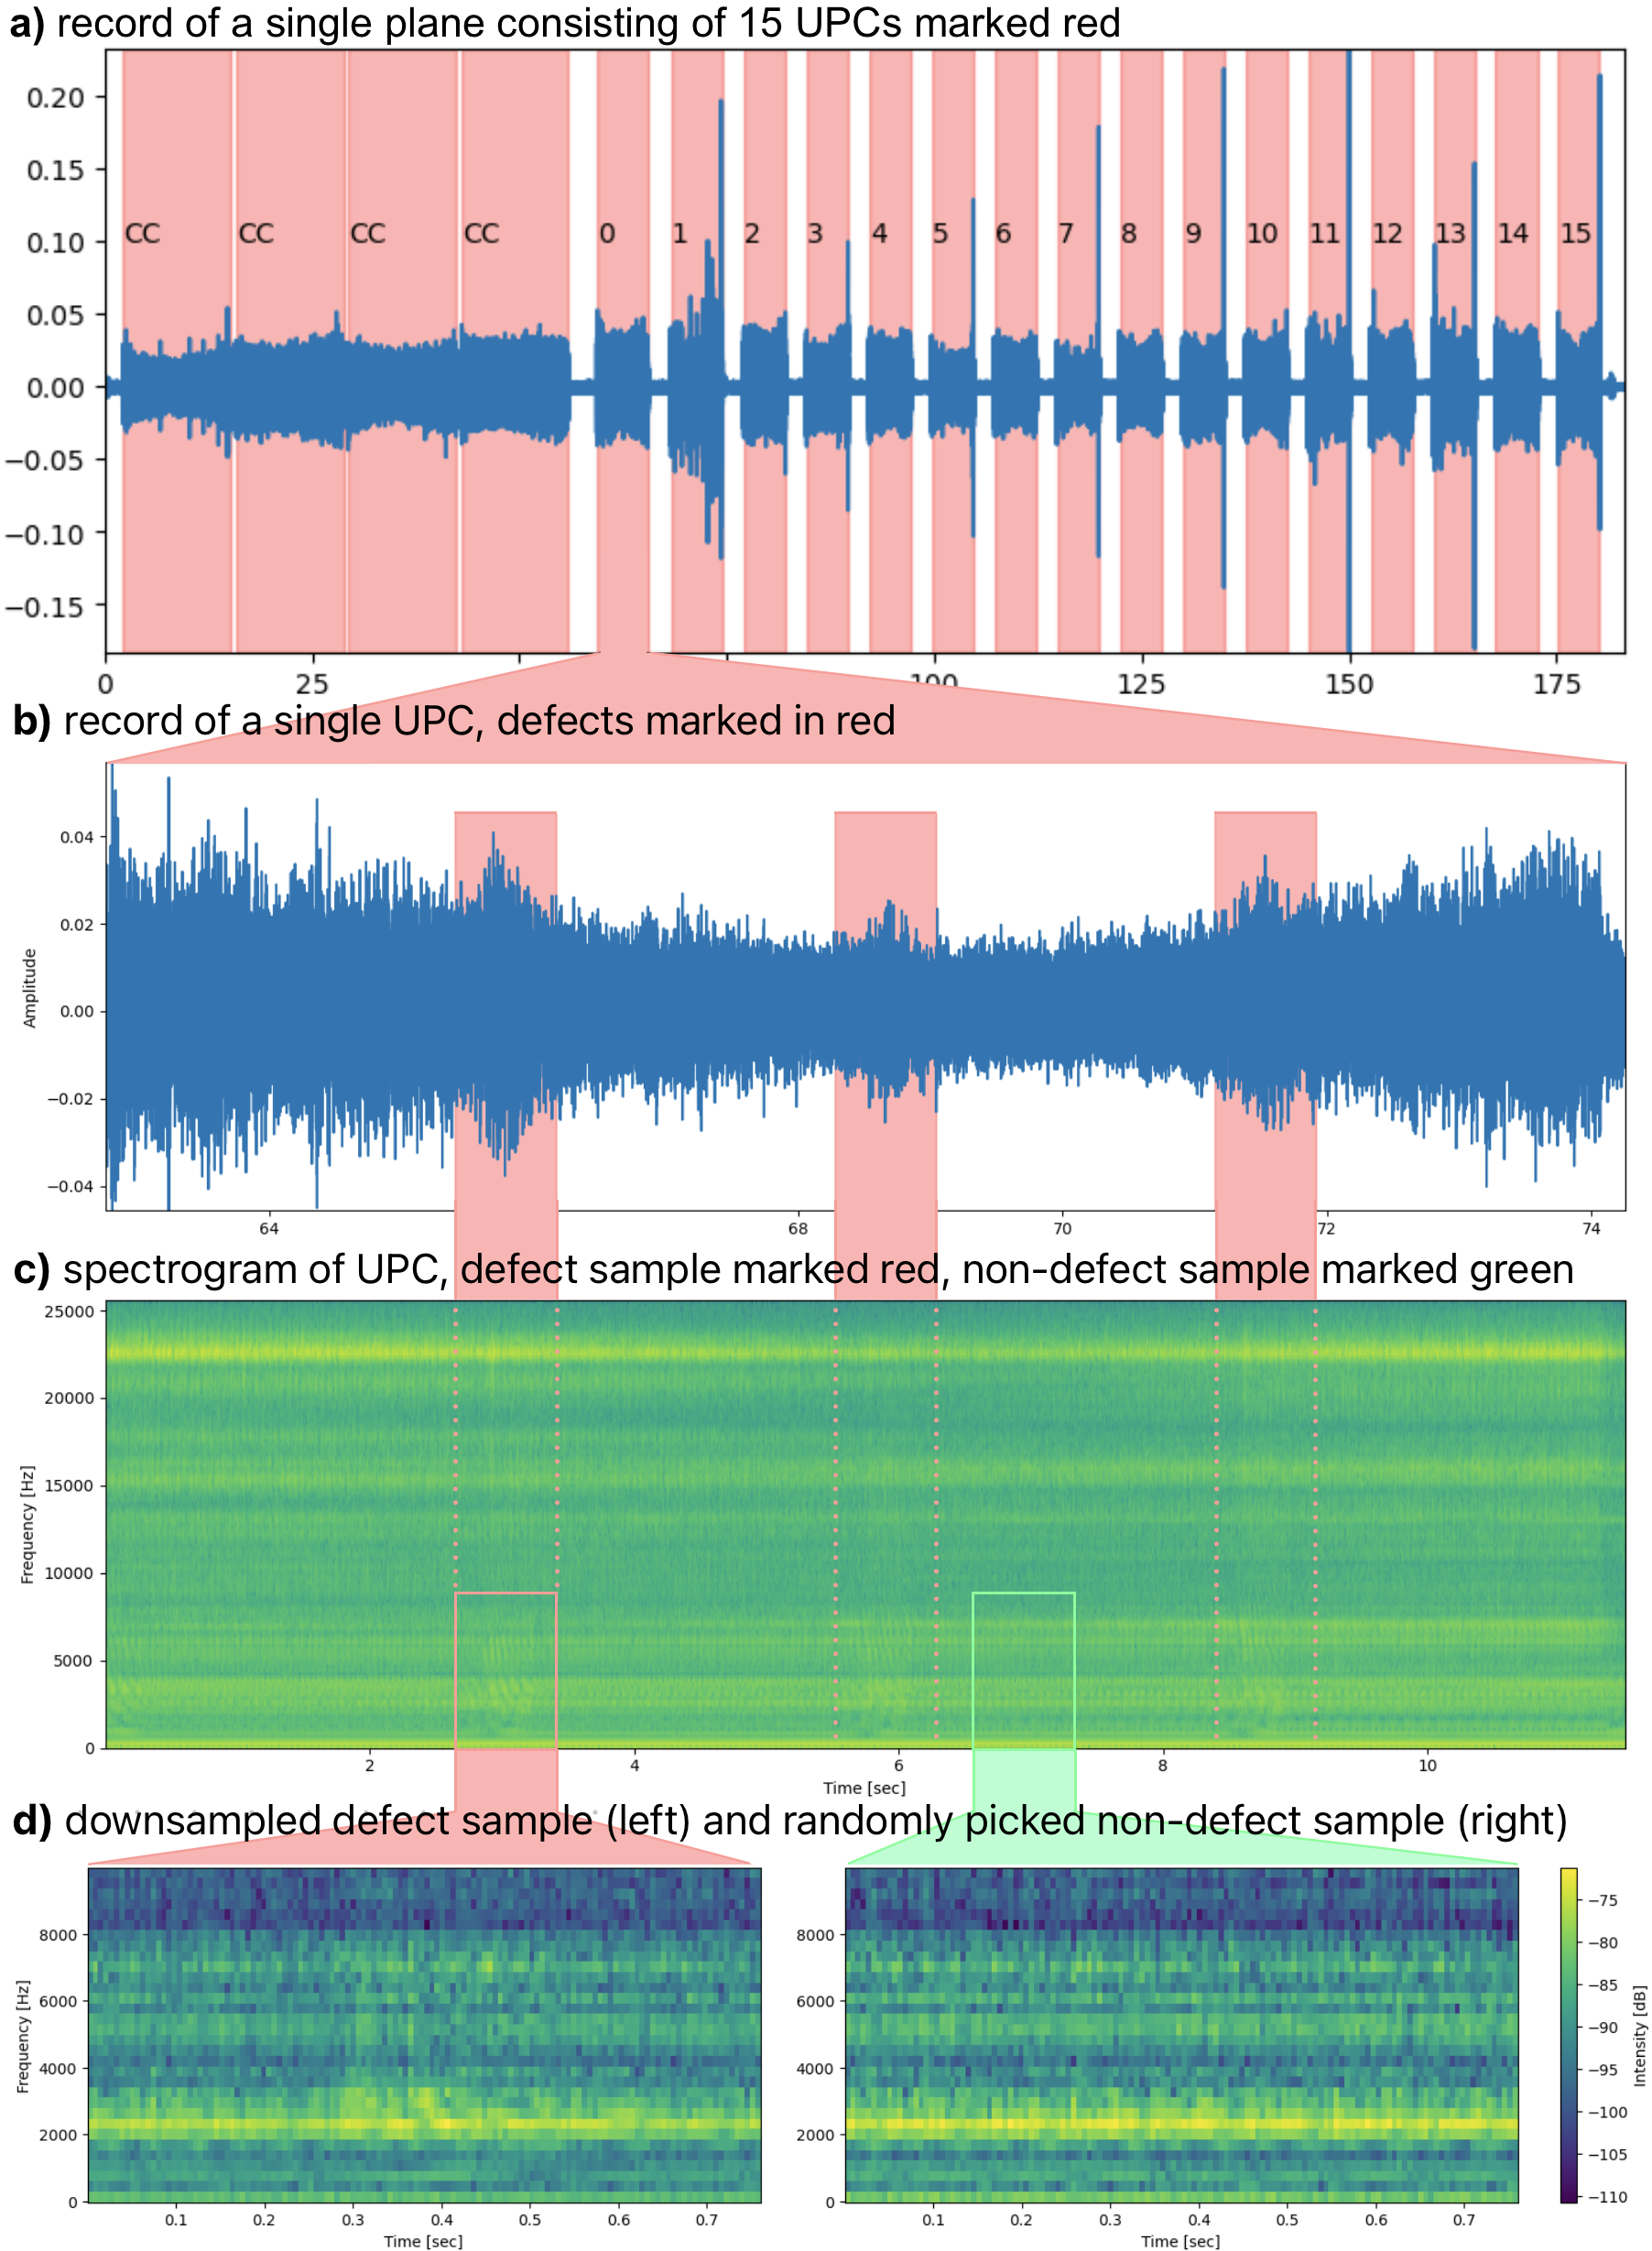
\includegraphics[width=0.99\linewidth]{dataset_gen.png}
    \caption{High-Level Concept}
    \label{Fig_ConceptDiagram}
\end{figure*}



\subsection{Experiment pipeline}
\vspace*{-\baselineskip}
neee eher net

\subsection{Experiment setup}
\vspace*{-\baselineskip}
DoE -> static gocode lines (drawing) 
in python, auf emco, ...


\subsection{ML model}
\vspace*{-\baselineskip}
üaspdfij

 
%=====================================================================
\section{Validation}
\begin{note}
	...and evaluation

\end{note}
%=====================================================================
\section{Conclusion}
\begin{note}
	and futere recommendation (halbe seite)
	
\end{note}





%=====================================================================
%=====================================================================
%% For references without a BibTeX database:
% JO bibliography
%\printbibliography               %biblatex -nope!
\bibliographystyle{elsarticle-num} %elsevierspecific -yep!
\bibliography{Bibliography.bib} %natbib %elsevier is based on natbib -so yep!

\end{document}
